\chapter{Formal Model}
\label{modelappendix}

The game has two rounds of play, each with four stages.\footnote{The two rounds of action generates complex notation. In the appendix, the first super/subscript number indicates the round in which the action occurred and the second indicates the case. So, $\act{1,2}$ represents the second case of the first round action proposal.} The actions formalize the theory's intuition that operational decisions require the assent of both the organization's leaders, who set and guide a strategic vision, and the rank-and-file who will ultimately carry out the actions. The need for internal agreement gives rise to an internal bargaining process in which leaders will explicitly or implicitly adjust to the actions that their followers will support.

The game that follows formalizes this process and extends the decision tree backwards to the point at which a Leader chooses whether or not to recruit, knowing that the new members will eventually wield influence.

Thus, each round proceeds as follows:

\begin{enumerate}
\item Leader recruits or not
\item Recruit accepts membership offer or not
\item Leader proposes a new activity
\item Recruit accepts or rejects the activity
\item The activity succeeds or fails, with a probability proportional to the level of resources that the Recruit brings to the organization.
\end{enumerate}

Figure~\ref{fig:extform} depicts one round of the game in extensive form.
\begin{figure}
  \centering
  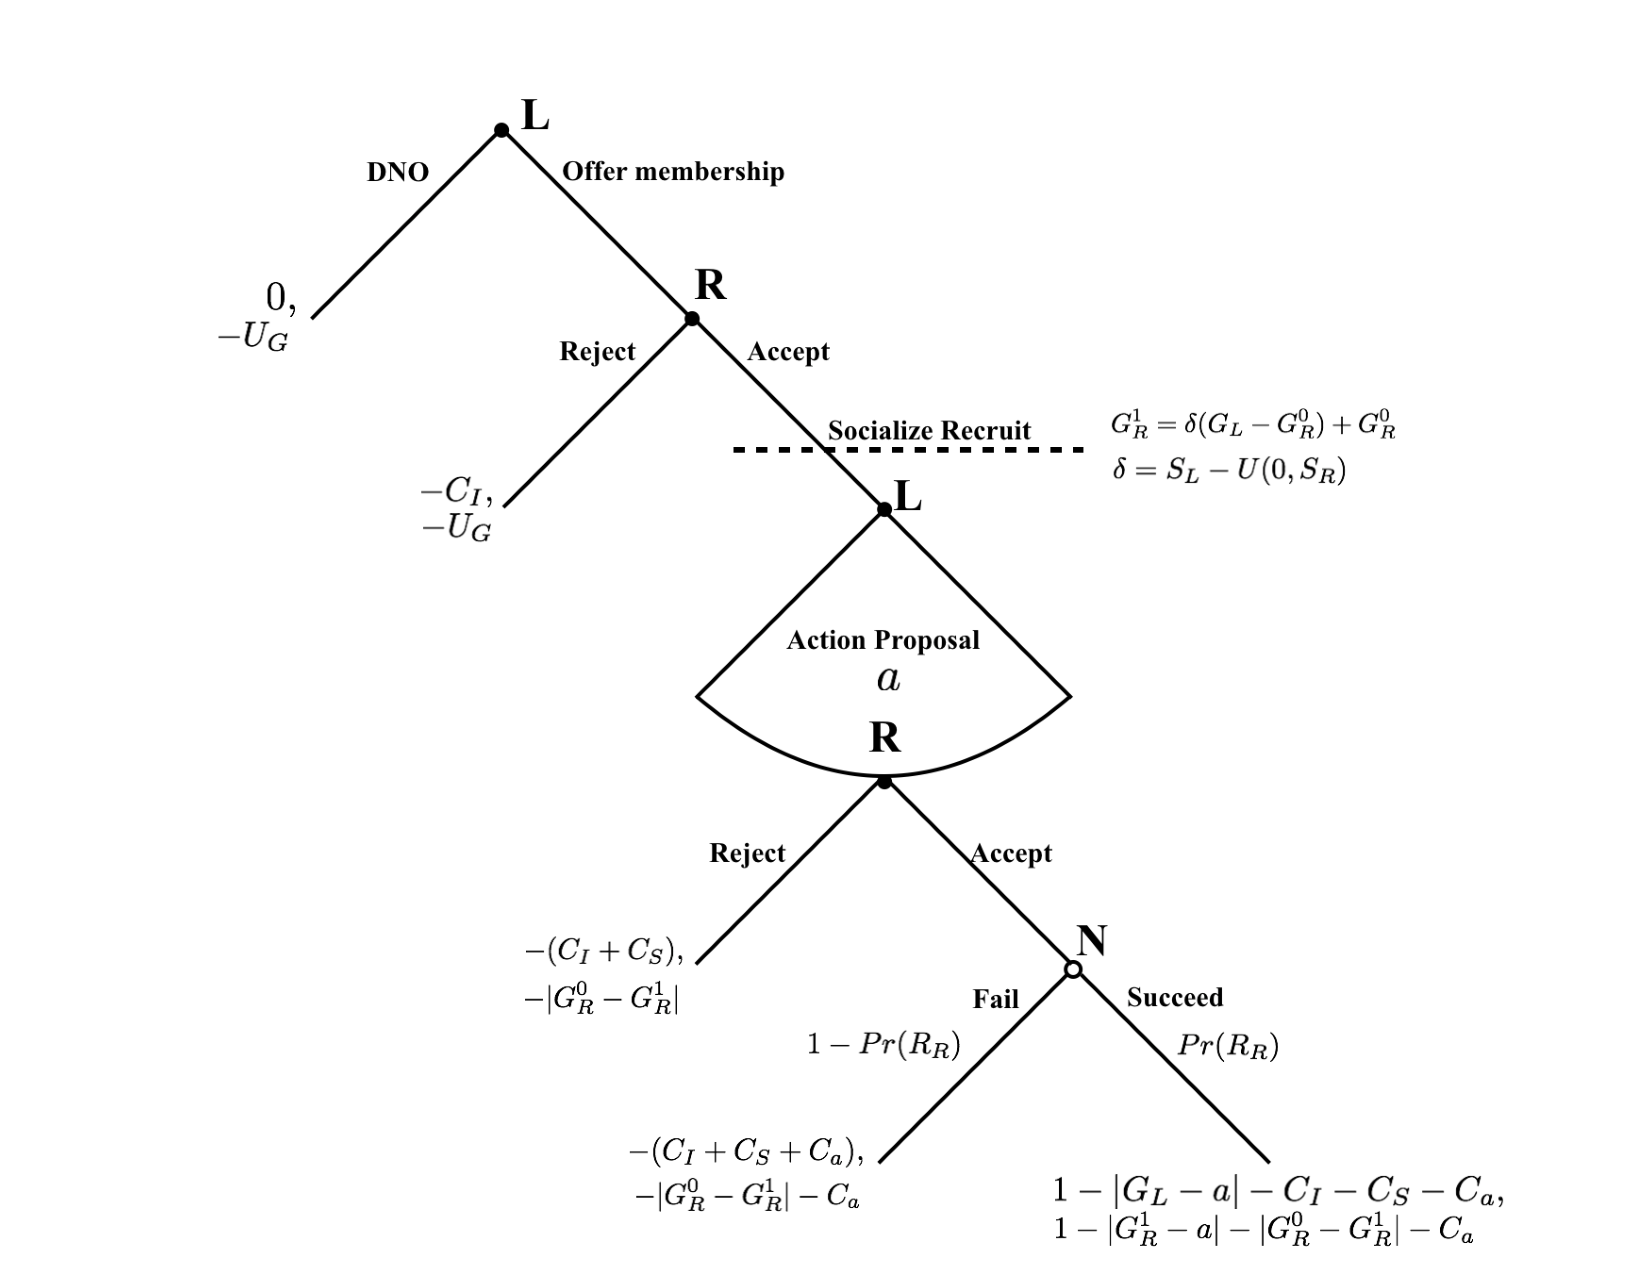
\includegraphics[width=.85\columnwidth]{../Pictures/RecruitGame_Round1.pdf}
  \caption{Recruitment Game, Extensive Form}
  \label{fig:extform}
\end{figure}

The solution concept is backwards induction. This is appropriate because the game is one of complete information and two rounds of play. Although simple, designing the game as one of complete information highlights the degree to which a Leader may
embark in an organization-transforming recruitment process
\textit{even knowing} that in equilibrium they will be obliged to updated their own eventual goal to include the preferences of the Recruit. 

To summarize the conditions of the equilibrium: the Recruit accepts ($a$) the proposed activity when their expected utility of a successful outcome ($s$) is at least as large as the expected utility of rejecting ($r$) the activity. The probability of success ($\ps{}$) is proportional to the level of resources ($R_{R}$) that the Recruit brings to the organization. The expected value of the recruit's socialization goals is $\egoal{1}$

\section*{Notation}

The equilibrium outlined below uses the following notation:
\begin{itemize}
\item Proposed actions are denoted with \textit{a}
\item Goals are denoted with a \textit{G}, with $G^{n}_{L}$ indicating
  the \textit{Leader's} goal for the $n^{th}$ update and $G^{n}_{R}$ indicating the \textit{Recruit's} goals for the $n^{th}$ updating.
  \item Costs are denoted with \textit{C}
  \begin{itemize}
  \item $C_{a}$ are the costs associated with the action.
  \item $C_{I}$ represents the Leader's costs to gather information about the potential Recruit.
  \item $C_{S}$ is the Leader's costs to socialize the new Recruit.
  \end{itemize}
    \item $\delta$ is the Leader's capacity to socialize the
      Recruit. It is function of the Leader's strength ($S_{L}$) and the Recruit's resistant capacity($S_{R})$.
      \item After the first round action, the Leader's goals update to represent a linear combination of the Leader's original goal and the previous round's action, weighted by $\alpha$. This updated goal is $\lgoal{1} = \alpha\lgoal{0}+(1-\alpha)\act{1}$
\end{itemize}

As the solution concept is backwards induction, analysis of the
conditions for equilibrium begin from the terminal node and work
backwards through the game.

\section{Second Round}

\textbf{Summary of equilibrium:}

%The leader recruits when $\lgoal{1}= \alpha \lgoal{0}+(1-\alpha)\act{1}$.
% By definition true, so not the equilibrium.

%has to be + between the two terms, or the updating doesn't work....
The Recruit accepts the offer if their expected utility after socialization is greater than the loss of utility for not being part of a group. This cutpoint occurs when: $|\rgoal{2}-\act{2}|\leq \gamma + \frac{U_{G}- |\delta(\rgoal{1}-\lgoal{1})|}{\ps{}}$, where $\gamma = 1- \frac{C_{a}}{P_{R}}$.  In the first round, the Recruit accepts with the same utility function, as it is a different recruit, and so from their perspective, the game is only a single round. Correspondingly, the Leader offers members if the cutpoint holds and the Leader's expected utility for the section action proposal is greater than zero ($EU^{2}_{L}(a^{*}_{2}) \geq 0$).

\underline{Full characterization of second round}

The Recruit's expected utility is: $EU^{2}_{R} = \ps{}(1- |\rgoal{2}- \act{2}| - \cost{} - |\rgoal{1}-\rgoal{2}|)$. They accept the action proposal $\act{2}$ if $EU^{2}_{R} \geq |\rgoal{1} - \rgoal{2}|$ or $P(R)[1- |\rgoal{2}- \act{2}| \geq \cost{}]$

In order for the Leader to propose an action the action must be chosen such that $\ps{}[1-|\lgoal{1} - \act{2}|] \geq \cost{}$ and $\ps{}[1-|\rgoal{2}- \act{2}|] \geq \cost{}$. Given this constraint, and the Recruit's acceptance cutpoint, the Leader chooses an action proposal, \act{2}, to maximize $\ps{}[1 -|\lgoal{1}-\act{2}|- \cost{} - \infocost{} - \socialcost{}]$. 

The Leader's maximization produces two cases:\\
Case (1): $\rgoal{1} \leq \lgoal{1}$\\
Case (2): $\rgoal{1} > \lgoal{1}$\\
In Case (1) if $|\lgoal{1}- \rgoal{2}-\gammacust| \leq \gammacust$, then $|\lgoal{1} - \act{2}| \leq \gammacust$ and $|\rgoal{2}- \act{2}| \leq \gammacust$ and  $\act{2} = min(\lgoal{1}, \rgoal{2} + \gammacust)$\\
If not, $\act{2} = \lgoal{1}$

In Case (2) if $|\rgoal{2} - \lgoal{1}- \gammacust| \leq \gammacust$,  $\act{2} = max(\lgoal{1}, \rgoal{2}-\gammacust)$\\
If not, $\act{2} = \lgoal{1}$\\

Moving up the game tree, the Recruit accepts the offer of membership if their expected utility from the action proposal $\act{2}$ is at least as high as their expected utility from being in the group. At this decision, the Recruit accepts if $EU^{2}_{R} \geq U_{G}$. 
This decision takes into account the expected effects of socialization, and so the potential Recruit agrees to join the group when $\rgoal{2}= \delta(\lgoal{1}- \rgoal{1}) + \rgoal{1}$ and  $|\lgoal{1}-\rgoal{2}|= |\delta(\rgoal{1}-\lgoal{1})|$. 

Combining the point at which the Recruit agrees to join the group and their expected level of socialization, the Recruit joins when:\\ $\ps{} (1-|\rgoal{2}- \act{2})|\geq \cost{} - U_{G} + |\delta (\rgoal{1} - \lgoal{1})|$\\
This condition simplifies to: 
$|\rgoal{2}- \act{2}| \leq \gammacust + \frac{U_{G} -|\delta(\rgoal{1}-\lgoal{1})|}{\ps{}}$

The Leader offers membership if the recruit will accept, and if the $EU_{L}^{2}(\act{2}) \geq 0 $

\underline{Full characterization of first round}\\
 
 The Leader selects an action proposal such that the action will maximize  $EU^{1}_{L}= \ps{}(1-|\lgoal{0}- a^{*}|) - \infocost{} -\socialcost{}- \cost{} -|\lgoal{1} - \lgoal{0}|$

Because the Leader proposes an action, $a^{*}_{1}$, that will be accepted by the Recruit, the expected utility becomes:\\
$\ps{}(1-|\lgoal{0}- \act{1}|)- \infocost{} - \socialcost{} -\cost{}- | \lgoal{1}-\lgoal{0}| \geq - \infocost{} - \socialcost{}$.

Replacing $\lgoal{1}$ with $\alpha\lgoal{0}+ (1-\alpha)\act{1}$ allows the equation to be simplified to:\\
$\ps{}-[\ps{} + (1-\alpha)](|\lgoal{0}- \act{1}|)\geq \cost{}$\\
$|\lgoal{0}- \act{1}| \leq \frac{\ps{}- \cost{}}{[\ps{} + (1-\alpha)]}$

As the initial conditions to arrive at the first round recruiting stage are true (\textit{i.e.}: that the Leader wants to offer recruitment options that the potential Recruit will accept), this condition implies that $|\rgoal{1}- \act{1}|\leq \gammacust$ and, from the above, $|\lgoal{0}- \act{1}|\leq \frac{\ps{}- \cost{}}{[\ps{} + (1-\alpha)]}$.

This creates two situations for the Leader: (1) when $\rgoal{1}\leq \lgoal{0}$ and (2) when $\rgoal{1} > \lgoal{0}$.

In case (1), where $\rgoal{1} \leq \lgoal{0}$,  if $|\lgoal{0}- \rgoal{1} - \gammacust| \leq \frac{\ps{}- \cost{}}{[\ps{} + (1-\alpha)]}$, $\act{1} = min(\lgoal{0}, \rgoal{1} + \gammacust)$  If not, $\act{1} =\lgoal{0}$.

In case (2),  $\rgoal{1} > \lgoal{0}$. In this case $\act{1}= max(\lgoal{0}, \rgoal{1}- \gammacust)$ when $|\rgoal{1}- \lgoal{0} - \gammacust| \leq \lgammacust$. If not, $\act{1} =\lgoal{1}$. If this case is not satisfied, the recruit accepts according to the same condition as in the second round: $|\rgoal{2}- \act{1}| \leq \gammacust + \frac{U_{G} -|\delta(\rgoal{1}-\lgoal{1})|}{\ps{}}$

Finally, the Leader initiates the recruitment cycle when: the Recruit will accept and $EU_{L} \geq 0$ where the expected utility of the Leader is: $EU^{1}_{L}= \ps{}(1-|\lgoal{0}- \act{1}|) - \infocost{} -\socialcost{}- \cost{} -|\lgoal{1} - \lgoal{0}|$